
In this chapter, we evaluate our quantification model and inference algorithms on simulated datasets with constant expected degradation rates and real direct RNA-seq datasets with sequencing spike-ins. 

\section{Read alignment}

Simulated and real reads were aligned with minimap2 (v.2.17-r941) \cite{Minimap2018, Minimap2021}, a popular aligner for long reads. For alignment to the genome, we used the flags \texttt{-ax splice -uf -k14} that take into account splicing and forward strand alignment for ONT direct RNA-seq as recommended by minimap2 developers. For alignment to the transcriptome, we use default flags \texttt{-ax map-ont -N10} for mapping ONT reads, keeping 10 secondary alignments due to similarities in transcript isoform sequences. We used the same genomic or transcriptomic alignments across the tools, depending on which is required as input.   

\section{Model variations}

We compare two variations of our model based on the read length-isoform agreement:

\paragraph{Deg. EM (exact)} We ran our model with the exact read length-isoform agreement model (Eqn. \ref{eq:read-iso-agreement}) and provided the known degradation rate to the model for inference. This is of course unrealistic, since in real data, the degradation rate is not known \textit{a priori} and there is no bound on the maximum read length (i.e., the degradation rate is not constant). Nevertheless, this serves as a useful sanity check that our approach works. 

\paragraph{Deg. EM (emp.)} The second variation of our model uses the empirical read length-isoform agreement model (Eqn. \ref{eq:emp-rlia}) and estimates the degradation rate per base from the data. This variation has no limitation on the maximum read length nor constraints on the degradation rate. 

\section{Methods for benchmarking}

We benchmark our model against three existing methods for transcript quantification from long-read RNA-seq. 

\paragraph{Bambu} Bambu \cite{Bambu2022} is a method for reference guided transcript discovery and quantification for long read RNA-seq data. Crucially, Bambu is one of the few existing long-read quantification methods that models degradation bias. For benchmarking, we ran Bambu (v.2.0.6) without transcript discovery. For transcript quantification, we ran Bambu with bias correction (default) and without bias correction (\texttt{degradationBias=FALSE}). We used the defaults for all other parameters.

\paragraph{FLAIR} Full-Length Alternative Isoform analysis of RNA (FLAIR) \cite{Tang2020} is a method for correction, isoform definition and alternative splicing analysis of long reads. For benchmarking, we ran FLAIR (v.1.5.1) with the modules \texttt{correct}, \texttt{collapse} and \texttt{quantify}. When running FLAIR on simulated data, we set \texttt{--support 1} for FLAIR \texttt{collapse}, keeping isoforms that are supported by minimally one read (default=3).  

\paragraph{NanoCount} NanoCount \cite{Gleeson2021} is a method for quantifying isoform abundance from ONT direct RNA-seq data. Of the three methods listed here, it is the most comparable to our model as it is tailored for direct RNA-seq and uses an expectation maximization algorithm for estimating isoform abundance estimates. For benchmarking, we ran NanoCount (v.1.0.0.post6) with default parameters.

\section{Evaluations on simulated data}\label{sec:eval-sim}

To evaluate our model's ability to correct for degradation bias, we simulated five datasets for a range of degradation rates $\mathbb{E}[d]\in\{0.05,0.1,0.2,0.4,0.5\}$ (Appendix \ref{ap:sim-deg-reads}). In addition, we simulated reads for artificial novel isoforms that are modified by dropping exons from the 5' end of selected reference isoforms, termed \textit{subset} isoforms (Appendix \ref{ap:gen-novl-iso}, Fig. \ref{fig:app-a-1}). This increases the proportion of multi-mapping reads and makes correcting for degradation bias crucial for accurate transcript quantification. 

The read counts for simulation follow a negative binomial distribution, which is often used for modeling RNA-seq counts and other count data that is over-dispersed, i.e., where the assumption of equal mean and variance is not held \cite{Cameron2013, Anders2010, Robinson2010}. We parameterise the distribution with the mean $\mu$ and a dispersion parameter $\alpha$ such that the variance is given by $\mu+\alpha\mu^2$. This is the same parameterisation used in \cite{Robinson2010}. To ensure that the negative binomial is a valid choice of distribution, we fit discrete distributions to the counts returned by existing methods on real long-read RNA-seq data, and find that the negative binomial provides a better fit to the data compared to the Poisson distribution (Appendix \ref{ap:count-dist}).   

\subsection{Comparisons between model variations}

In this section, we compare the Deg. EM (exact) and Deg. EM (emp.) models based on the isoform abundance estimates obtained. We compare these estimates against the simulated ground truth based on Spearman correlation (SCC), normalized root-mean-squared error (NRMSE) and median relative difference (MRD). Explanations of these metrics can be found in Appendix \ref{ap:eval-metrics}.  

Both variations of the model perform comparably well on the simulated data, achieving SCC $>$ 0.775 across all five simulated datasets with low NRMSE and MRD. Table \ref{tab:summary-1} shows the mean of each metric across the five datasets for all and subset isoforms. We first note that performance on the subset isoforms is slightly poorer compared to that on all isoforms, for both variations and across metrics. This is expected as there is more ambiguity in read assignment with the subset isoforms. 

% Table generated by Excel2LaTeX from sheet 'sec-4-1-table'
\begin{table}[htbp]
\centering
  \resizebox{\columnwidth}{!}{%
\begin{tabular}{|l|P{2cm}|P{2cm}|P{2cm}|P{2cm}|P{2cm}|P{2cm}|}
\cline{2-7}    \multicolumn{1}{c|}{} & \multicolumn{3}{c|}{All isoforms} & \multicolumn{3}{c|}{Subset isoforms} \bigstrut\\
\hline
Method & SCC   & NRMSE & MRD   & SCC   & NRMSE & MRD \bigstrut\\
\hline
Deg. EM (exact) & 0.848 & 0.429 & \textbf{0.015} & \textbf{0.813} & \textbf{0.44} & \textbf{0.127} \bigstrut\\
\hline
Deg. EM (emp) & \textbf{0.852} & \textbf{0.416} & 0.016 & 0.778 & 0.448 & 0.285 \bigstrut\\
\hline
\end{tabular}%
}
\caption[Summary of metrics across simulated datasets for model variations]{Summary of metrics across simulated datasets for model variations. We report the mean SCC, NRMSE and MRD across the five datasets for all isoforms and subset isoforms separately. Bold values indicate the best performance for each column.}
\label{tab:summary-1}
\end{table}%

Next, we examine the performance on each dataset separately for all and subset isoforms (Fig. \ref{fig:4-1-scc-nrmse}). Across all isoforms, the variations perform extremely similarly. In contrast, on the subset isoforms, the exact model dominates the empirical model in SCC and MRD. This is expected, as estimations with the empirical cumulative distribution function introduce noise to the estimates. Conversely, the exact model is formulated exactly to work on the data. 

To investigate these differences further, we visualised estimates and fitted a kernel density estimate on the subset isoforms only for datasets with degradation rates 0.2 and 0.5 (Fig. \ref{fig:4-1-scatter}). On a dataset with relatively lower degradation rate (0.2), the exact model performs qualitatively well, with the density of points over the diagonal (Fig. \ref{fig:4-1-scatter}a), while the empirical model underestimates counts for certain isoforms (Fig. \ref{fig:4-1-scatter}b). We see similar results in datasets with higher degradation rates (0.5) where the variance in the estimates returned by the exact model is lower (Fig. \ref{fig:4-1-scatter}c) compared to the empirical model, where the counts are more diffuse about the diagonal (Fig. \ref{fig:4-1-scatter}d). This deviation from the diagonal also explains the increase in MRD in the empirical model for larger degradation rates compared to the exact model (Fig. \ref{fig:4-1-scc-nrmse}).

Based on our analyses in section \ref{sec:deg-est}, we observed that average degradation rates in real direct RNA-seq data tend to be in the range of 0.1-0.2. In this range, the two variations perform comparably, and have a high SCC with each other ($\mathbb{E}[d]$=0.1, SCC=0.962, $\mathbb{E}[d]$=0.2, SCC=0.962).  

\begin{figure}[H]
    \centering
    \includegraphics[width=0.9\textwidth]{figures/sec-4-1-scc-nrmse.png}
    \caption[SCC, NRMSE and MRD across simulated datasets for model variations]{SCC, NRMSE and MRD across simulated datasets for model variations. Here, each point is a dataset with constant expected degradation $\mathbb{E}[d]=\{0.05,0.1,0.2,0.4,0.5\}$. \textbf{a.} SCC on all isoforms. \textbf{b.} SCC on subset isoforms. \textbf{c.} NRMSE on all isoforms. \textbf{d.} NRMSE on subset isoforms. \textbf{f.} MRD on all isoforms. \textbf{e.} MRD on subset isoforms.}
    \label{fig:4-1-scc-nrmse}
\end{figure}

\begin{figure}[H]
    \centering
    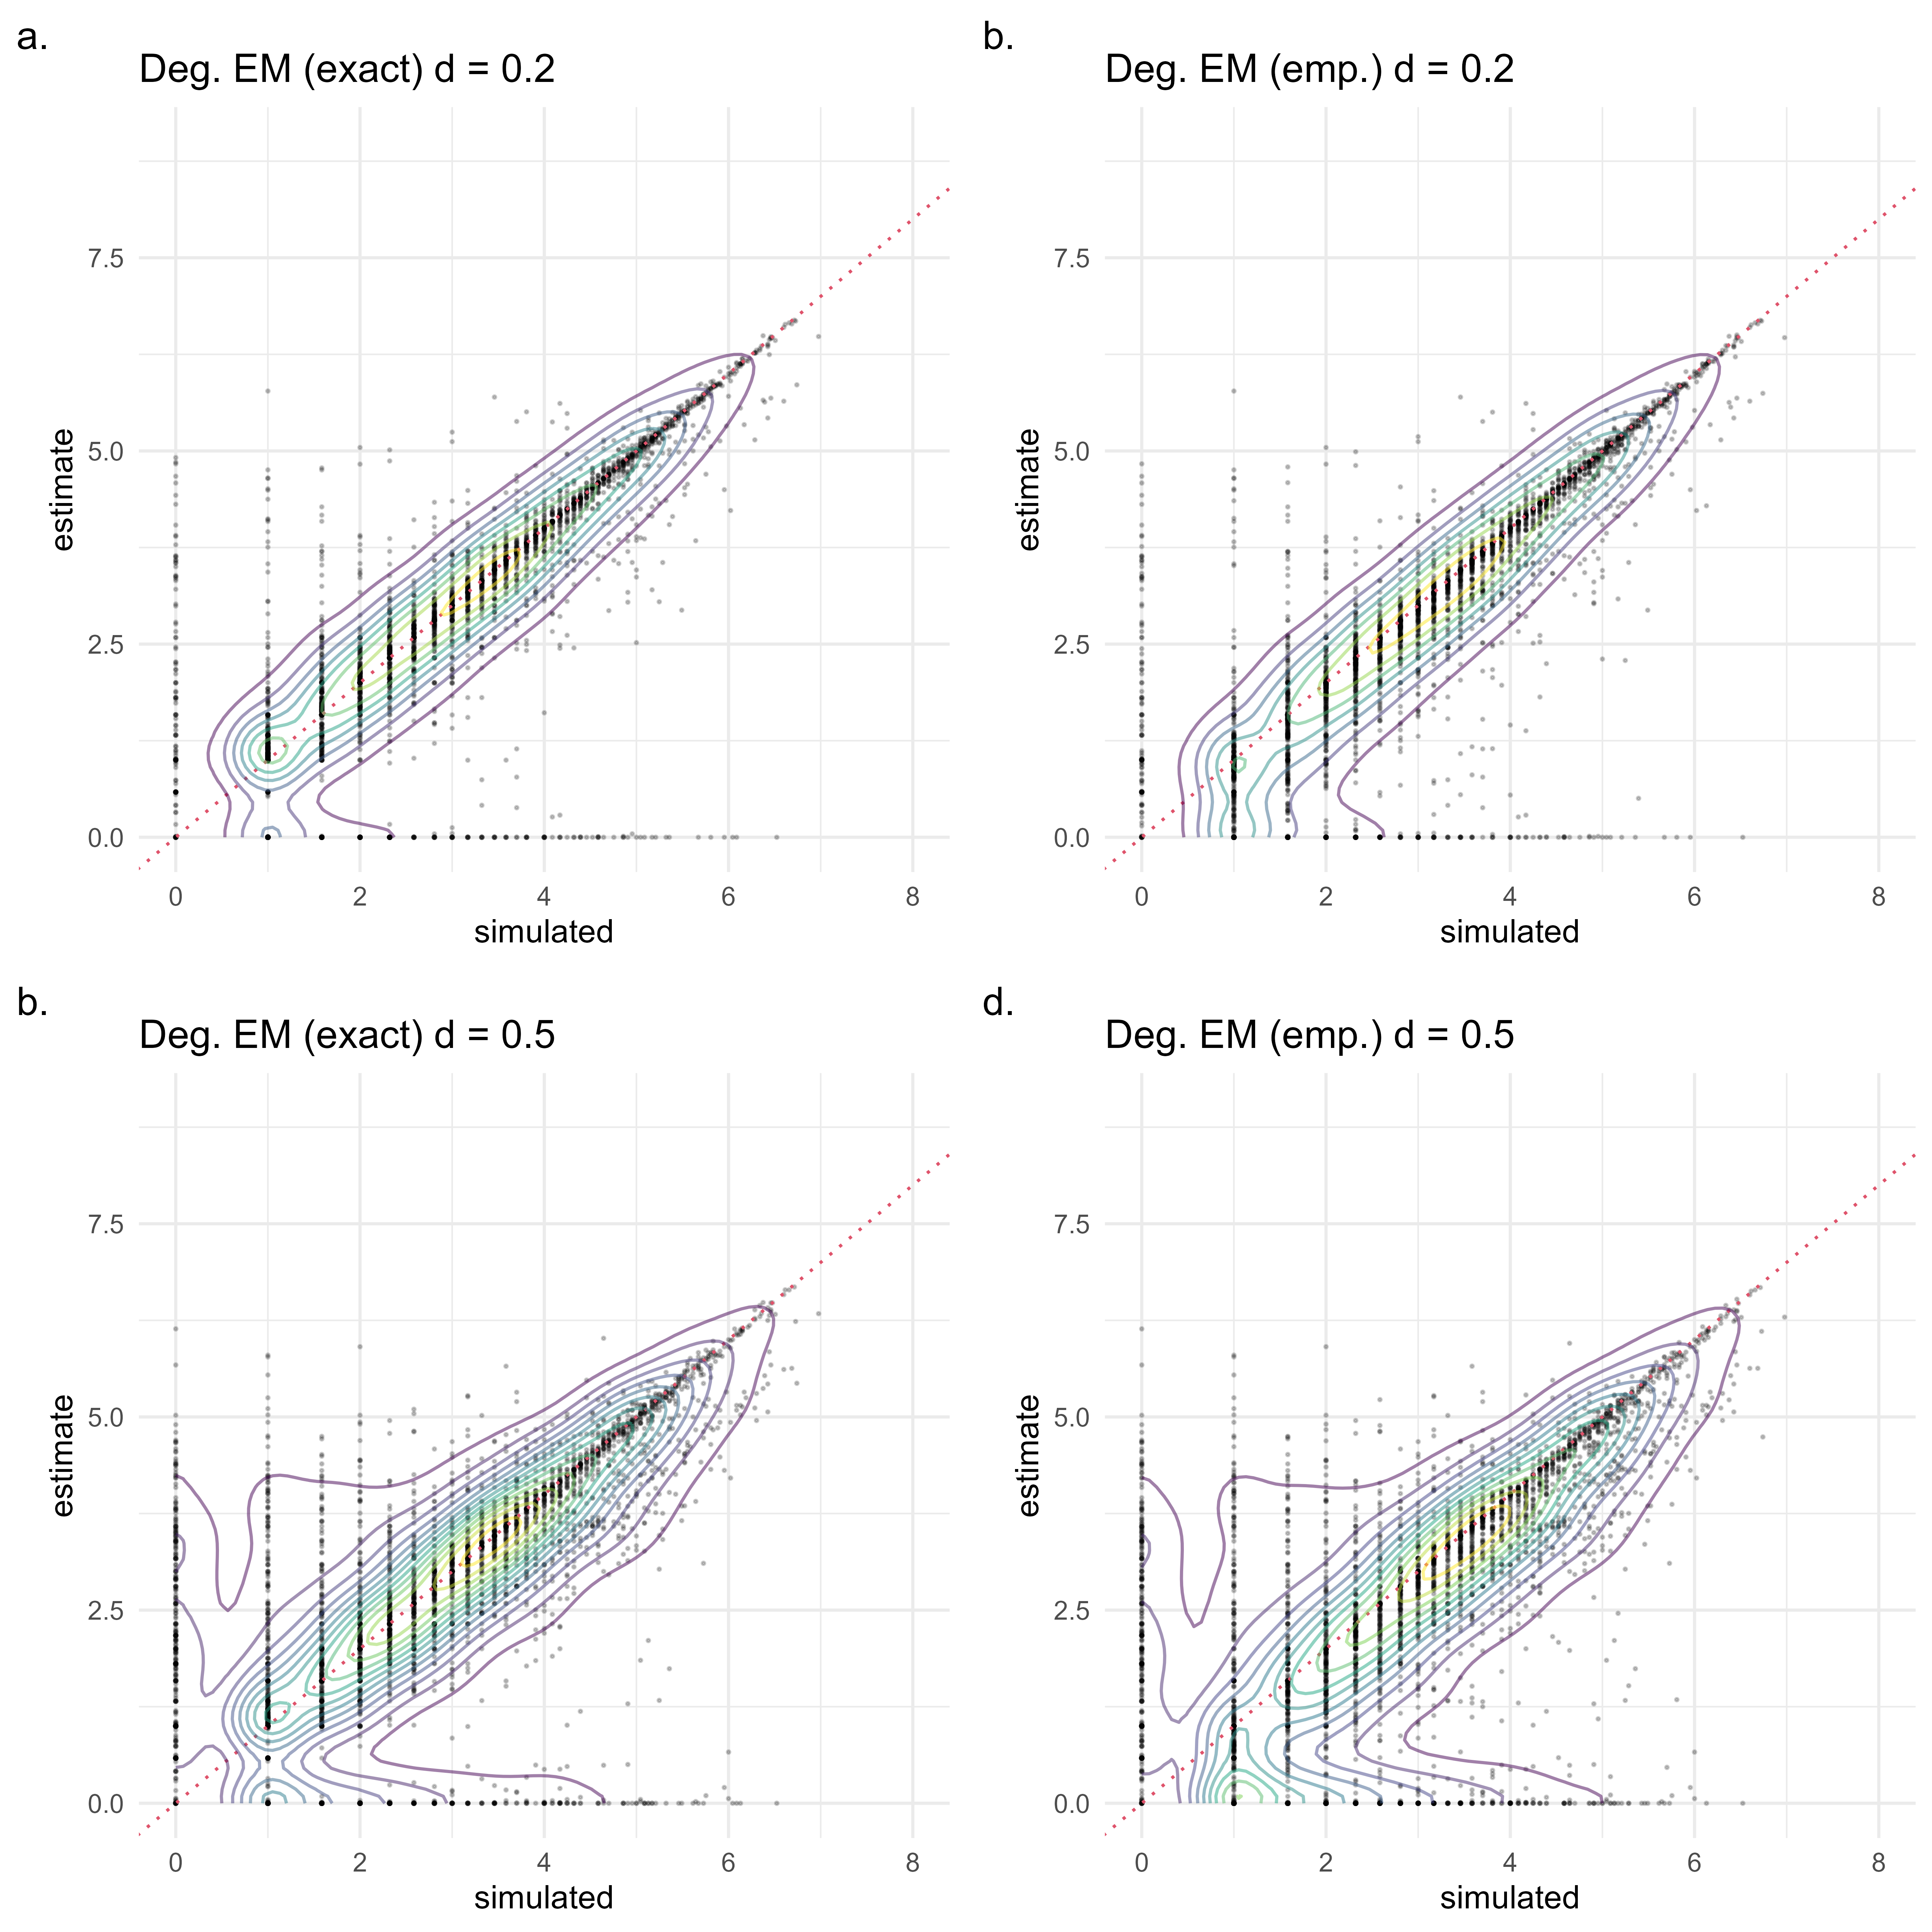
\includegraphics[width=\textwidth]{figures/sec-4-1-scatter-hard.png}
    \caption[Scatter plots across simulated datasets for model variations]{Scatter plots of the simulated and estimated counts on the log2 scale across simulated datasets with $\mathbb{E}[d]=0.2$ and $\mathbb{E}[d]=0.5$ for the exact and empirical model. \textbf{a.} Exact model with degradation 0.2. \textbf{b.} Empirical model with degradation 0.2. \textbf{c.} Exact model with degradation 0.5. \textbf{d.} Empirical model with degradation 0.5.}
    \label{fig:4-1-scatter}
\end{figure}

\subsection{Comparisons with existing methods}

We now benchmark our model against Bambu with and without bias modeling, FLAIR and NanoCount by comparing the estimates returned by each method with the simulated ground truth. We analyse counts for all isoforms that we included in the simulation and where the sum of counts across the methods was greater than zero. In addition, we make a distinction between methods that are \textit{bias-aware} (Deg. EM (exact), Deg. EM (emp.), Bambu) and methods that are \textit{bias-unaware} (Bambu (no bias), FLAIR, NanoCount). 

All methods perform reasonably well on the simulated data across all isoforms, achieving SCC $>$ 0.69 across all five simulated datasets (Table \ref{tab:summary-2}). NRMSE across the methods are comparable, but MRD for the other methods are about one order of magnitude larger than those attained by our model. However, we observe stark differences between the bias-aware and bias-unaware methods on the subset isoforms. In particular, bias-unaware methods perform considerably poorer on SCC and MRD than bias-aware ones (Table \ref{tab:summary-2}).    

\begin{table}[htbp]
\centering
\resizebox{\columnwidth}{!}{%
\begin{tabular}{|l|P{2cm}|P{2cm}|P{2cm}|P{2cm}|P{2cm}|P{2cm}|}
\cline{2-7}    \multicolumn{1}{r|}{} & \multicolumn{3}{c|}{All isoforms} & \multicolumn{3}{c|}{Subset isoforms} \bigstrut\\
\hline
Method & SCC   & NRMSE & MRD   & SCC   & NRMSE & MRD \bigstrut\\
\hline
Deg. EM (exact) & 0.86 & 0.423 & \textbf{0.011} & \textbf{0.834} & \textbf{0.431} & \textbf{0.104} \bigstrut\\
\hline
Deg. EM (emp.) & \textbf{0.863} & \textbf{0.41} & 0.012 & 0.801 & 0.439 & 0.241 \bigstrut\\
\hline
Bambu & 0.771 & 0.599 & 0.101 & 0.671 & 1.009 & 0.36 \bigstrut\\
\hline
Bambu (no bias) & 0.739 & 0.637 & 0.107 & 0.432 & 1.165 & 0.926 \bigstrut\\
\hline
FLAIR & 0.696 & 0.697 & 0.081 & 0.153 & 1.176 & 0.974 \bigstrut\\
\hline
NanoCount & 0.759 & 0.566 & 0.105 & 0.408 & 1.056 & 0.931 \bigstrut\\
\hline
\end{tabular}%
}
\caption[Summary of metrics across simulated datasets for different methods]{Summary of metrics across simulated datasets for different methods. We report the mean SCC, NRMSE and MRD across the five datasets for all isoforms and subset isoforms separately. Bold values indicate the best performance for each column.}
\label{tab:summary-2}
\end{table}%

Next, we examine the performance on each dataset separately for all the methods on all and subset isoforms separately (Fig. \ref{fig:4-2-scc-nrmse}). Both Deg. EM (exact) and Deg. EM (empirical) show better performance on all metrics compared to other methods across the datasets. We also note that Bambu with bias modeling improves the performance over Bambu without bias modeling across the whole range of degradation rates. In addition, Bambu's performance drops quickly as the degradation rate increases, as its degradation rate is purposefully calibrated or moderated to lower degradation rates. The authors note that this is to allow for comparisons across samples or replicates, as correction for different degradation rates across samples may result in technical variation which impact downstream analyses. We examine this claim based on reproducibility metrics on real data in the following section. For degradation rates commonly observed in real data (0.1-0.2), Bambu performs better compared to FLAIR and NanoCount on both SCC and NRMSE (Fig. \ref{fig:4-1-scc-nrmse}a,c). 

Bias-unaware methods perform poorly over the subset isoforms across the whole range of degradation rates. Interestingly, the MRD on subset isoforms for bias-unaware methods remained consistently high and was invariant across the range of degradation rates, while for bias-aware methods, the MRD was always lower compared to bias-unaware methods and increased with the degradation rate (\ref{fig:4-2-scc-nrmse}e). This demonstrates the importance of bias correction and illustrates the difficulty of correcting for degradation bias when the degradation rate is high.     

\newpage

\begin{figure}[H]
    \centering
    \includegraphics[width=0.9\textwidth]{figures/sec-4-2-scc-nrmse.png}
    \caption[SCC, NRMSE and MRD across simulated datasets for different methods]{SCC, NRMSE and MRD across simulated datasets for different methods. Here, each point is a dataset with constant expected degradation $\mathbb{E}[d]=\{0.05,0.1,0.2,0.4,0.5\}$. \textbf{a.} SCC on all isoforms. \textbf{b.} SCC on subset isoforms. \textbf{c.} NRMSE on all isoforms. \textbf{d.} NRMSE on subset isoforms. \textbf{f.} MRD on all isoforms. \textbf{e.} MRD on subset isoforms.}
    \label{fig:4-2-scc-nrmse}
\end{figure}

\newpage

\begin{figure}[H]
    \centering
    \includegraphics[width=0.9\textwidth]{figures/sec-4-2-scatter-hard.png}
    \caption[Scatter plots across simulated datasets for different methods]{Scatter plots of the simulated and estimated counts on the log2 scale across simulated datasets with $\mathbb{E}[d]=0.2$ for all methods. \textbf{a.} Deg. EM (exact) model. \textbf{b.} Deg. EM (emp.) model. \textbf{c.} Bambu with bias modeling. \textbf{d.} Bambu with no bias modeling. \textbf{e.} FLAIR. \textbf{f.} NanoCount.}
    \label{fig:4-2-scatter}
\end{figure}

\newpage

Finally, we visualised estimates and fitted a kernel density estimate on the subset isoforms for all methods on the dataset with a degradation rate of 0.2 (Fig. \ref{fig:4-2-scatter}), which we observe to be common in real data. On this dataset, bias-aware methods significantly improve over bias-unaware ones qualitatively (Fig. \ref{fig:4-2-scatter}a,b,c). In particular, without correcting for bias, Bambu (no bias), FLAIR and NanoCount (Fig. \ref{fig:4-2-scatter}d,e,f) severely underestimate the counts for subset isoforms to different extents, with FLAIR performing the worst.

\subsection{Runtime analysis}

We measured the end-to-end runtime taken for all methods (Fig. \ref{fig:runtime}) excluding the read alignment step. Bambu and FLAIR were run with 12 threads, while NanoCount and the current verison of our model do not implement parallelisation. Across the five datasets, NanoCount was the fastest, followed by Deg. EM (exact). Bambu and FLAIR performed similarly, though FLAIR had a much larger variance in the runtime. Even though the time complexity for both Deg. EM (exact) and Deg. EM (emp.) is $\mathcal{O}(N_A)$, where $N_A$ is the number of alignments, Deg. EM (emp.) is much slower than all other methods because calculation of the empirical read length-isoform agreement probabilities is computationally intensive. Even though the runtimes for the empirical model are longer, they are still tolerable in absolute terms, and come with improvements in accuracy for accurately quantifying degraded reads. Nevertheless, this is one area for improvement for future iterations of our model.  

\begin{figure}[H]
    \centering
    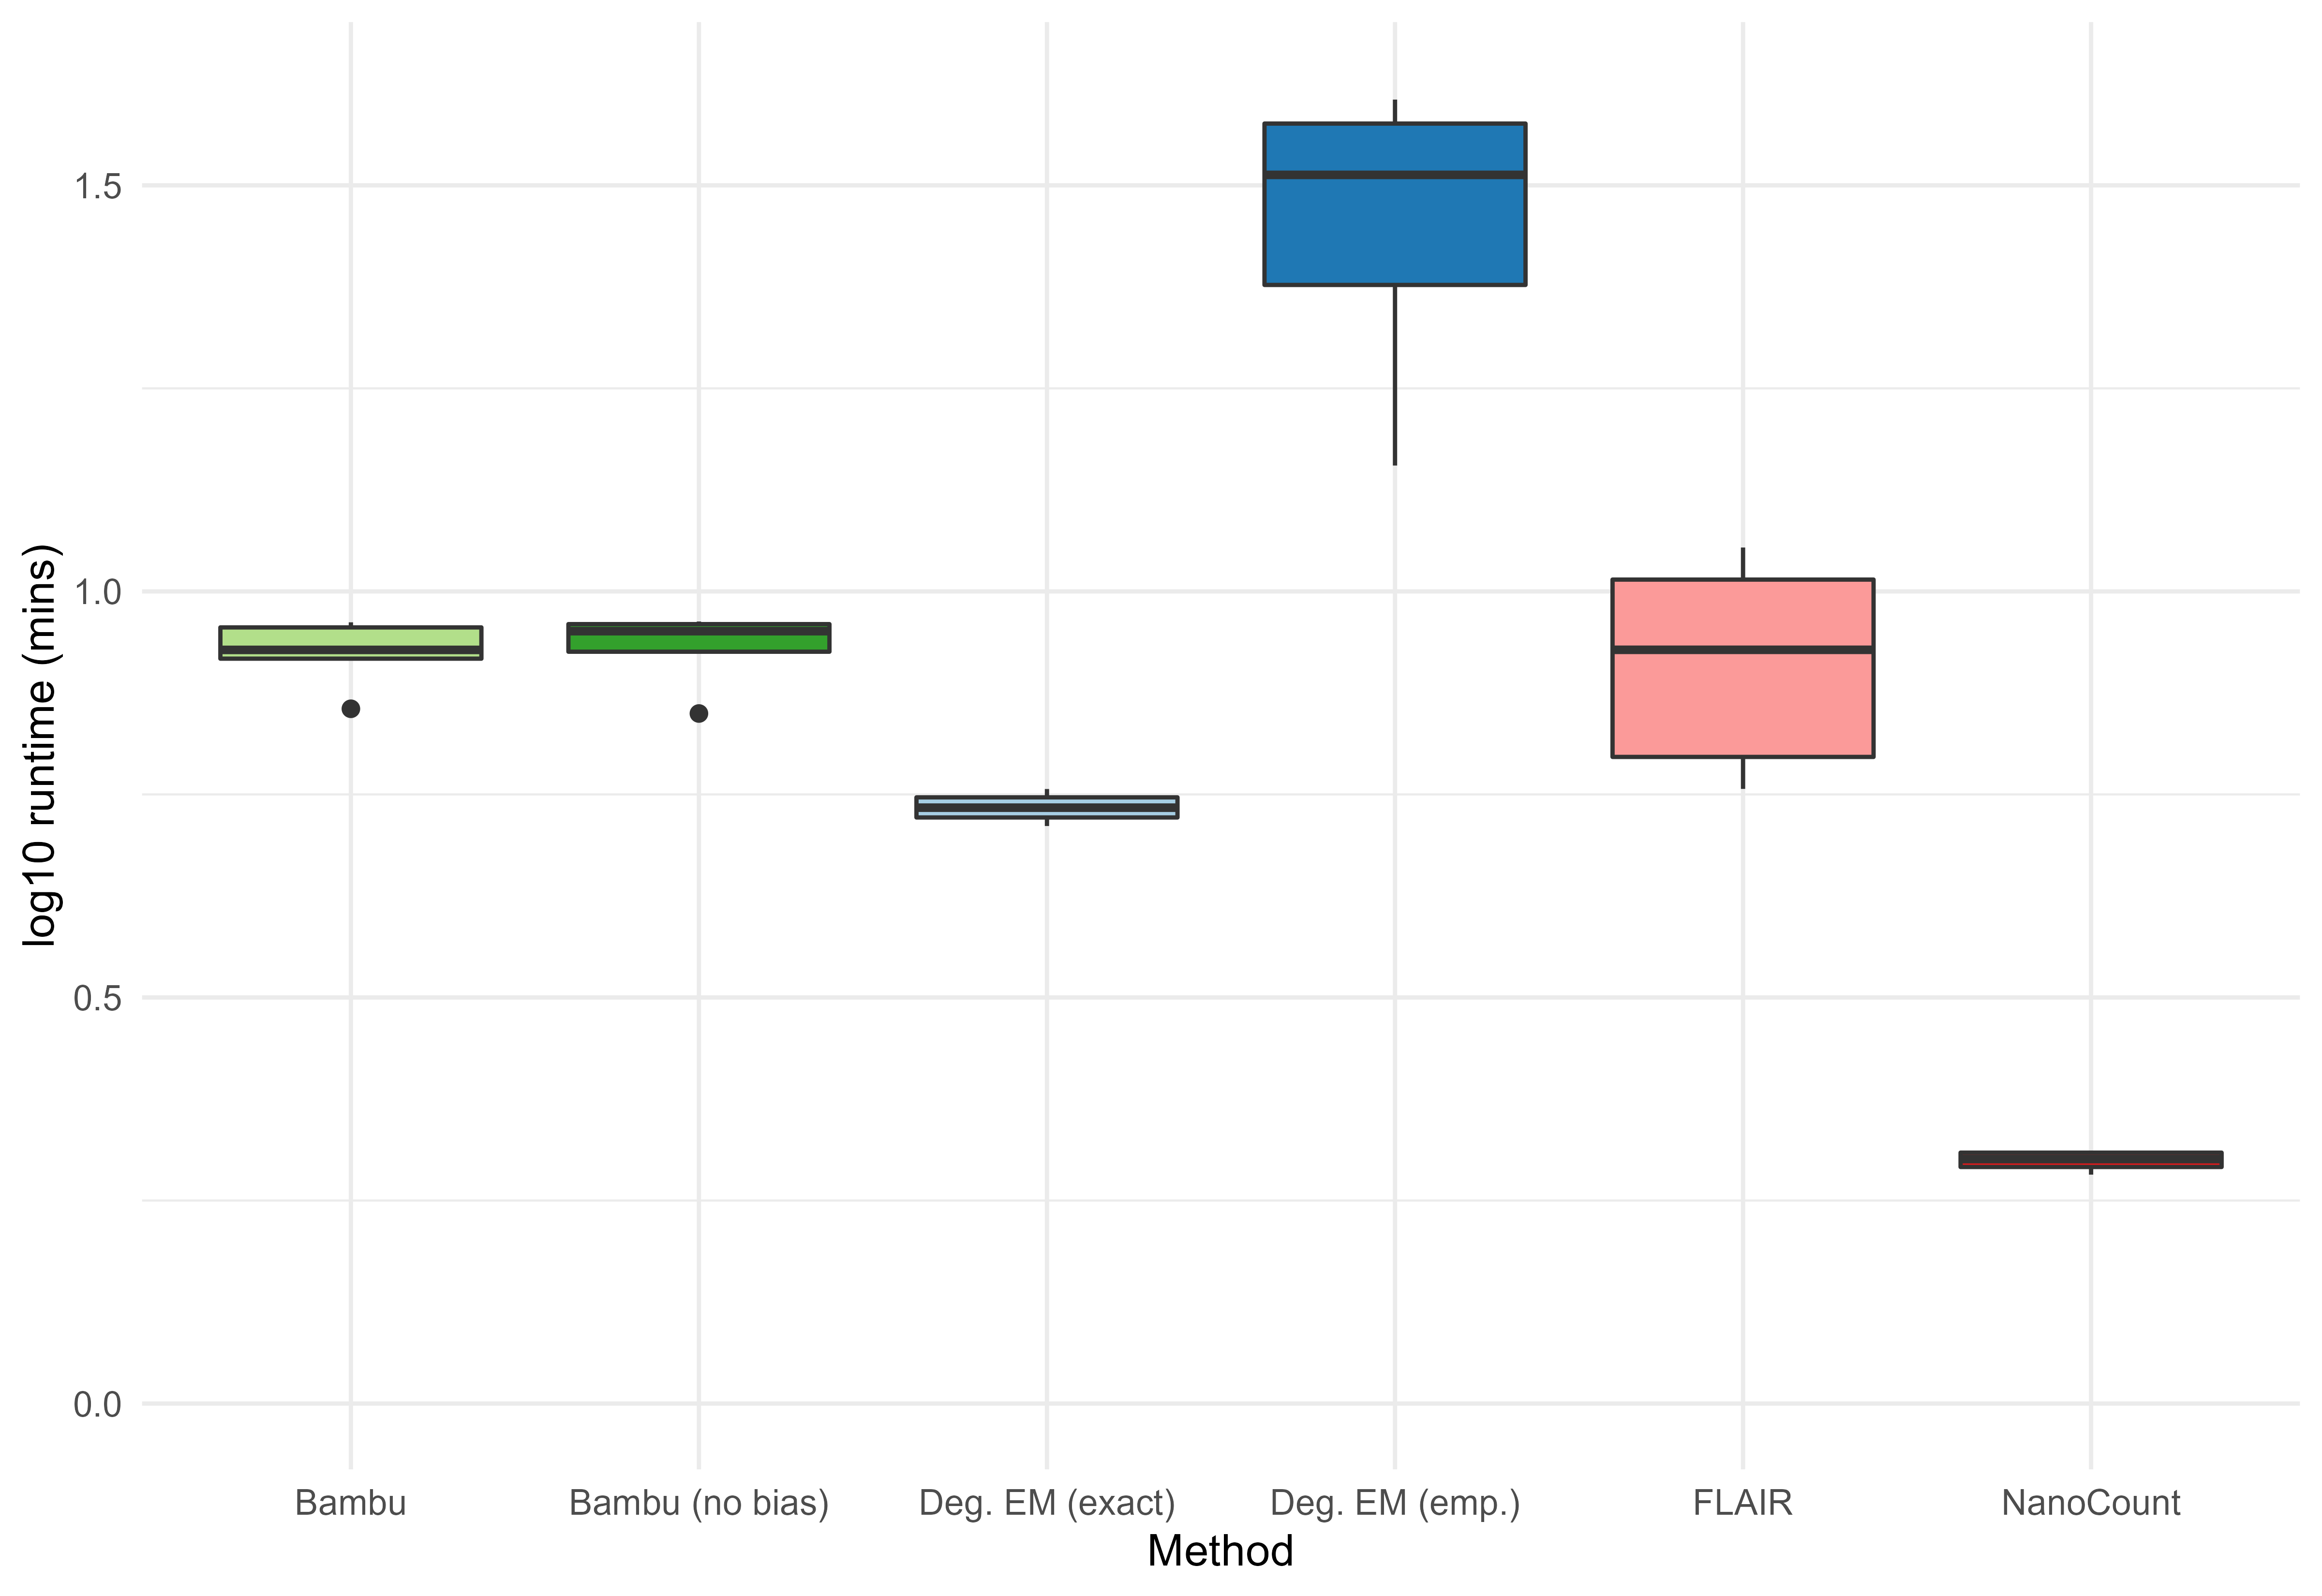
\includegraphics[width=0.825\textwidth]{figures/sec-4-runtime.png}
    \caption[Runtime across simulated datasets for different methods]{Runtime (mins) across simulated datasets for different methods. Times are log10 transformed.}
    \label{fig:runtime}
\end{figure}

\section{Evaluations on real data}

In this section, we evaluate Deg. EM (emp.), Bambu with bias modeling, and NanoCount on direct RNA-seq data from the SG-NEx project. In particular, we examine the performance of these methods on samples containing RNA sequencing spike-ins (Table \ref{tab-sgnex}). A subset of samples contains Spike-In RNA Variants (SIRVs) \cite{Lexogen20201} while another contains RNA sequins \cite{Sequins}. The expression of these spike-ins are supposedly known and can be used as a reference.   

\begin{table}[htbp]
  \centering
    \begin{tabular}{|p{2cm}|p{2cm}|p{2cm}|p{3.5cm}|}
    \hline
    Cell Line & Run & Replicate   & Spike-in \bigstrut\\
    \hline
    Hct116 & 1     & 3     & Sequin Mix A v1.0 \bigstrut\\
    \hline
    K562  & 1     & 4     & Sequin Mix A v1.0 \bigstrut\\
    \hline
    K562  & 1     & 5   & Sequin Mix A v1.0 \bigstrut\\
    \hline
    MCF7  & 1     & 4     & Sequin Mix A v1.0 \bigstrut\\
    \hline
    H9    & 1     & 2     & SIRV-4 \bigstrut\\
    \hline
    H9    & 1     & 3     & SIRV-4 \bigstrut\\
    \hline
    H9    & 1     & 4     & SIRV-4 \bigstrut\\
    \hline
    H9    & 2     & 2     & SIRV-4 \bigstrut\\
    \hline
    H9    & 2     & 3     & SIRV-4 \bigstrut\\
    \hline
    H9    & 2     & 4     & SIRV-4 \bigstrut\\
    \hline
    \end{tabular}%
  \caption[Description of SG-NEx direct RNA-seq samples.]{Description of SG-NEx direct RNA-seq samples. A subset of samples is spiked-in with Sequins while another is spiked-in with SIRV-4.}
  \label{tab-sgnex}
\end{table}%

\subsection{Empirical results on spike-ins}

First, we examine results on the RNA sequin spike-ins (n = 41 transcripts). For each of the four samples, we computed the SCC, NRMSE and MRD on the abundance estimates returned by each method (Fig. \ref{fig:sequin-metrics}). Deg. EM (emp.) achieved the highest median SCC, while NanoCount perform reasonably well with a median SCC $>$ 0.7. Bambu's performance was weighed down by an outlier (Fig. \ref{fig:sequin-metrics}a). NRMSE and MRD metrics show similar trends, with Deg. EM (emp.) achieving the lowest median NRMSE and MRD (Fig. \ref{fig:sequin-metrics}b,c).

We visualize the estimates and supposed concentrations of the sequins for the sample K562 replicate 5 run 1 (Fig \ref{fig:sequin-scatter}) which obtained close to median performance across the metrics for all methods. Qualitatively, Deg. EM and NanoCount achieve similar results, though in the latter, there is a slight overestimation of counts. Bambu underestimates the counts for a subset of lowly expressed sequins that results in a decrease in performance over the three metrics.  

\begin{figure}[H]
    \centering
    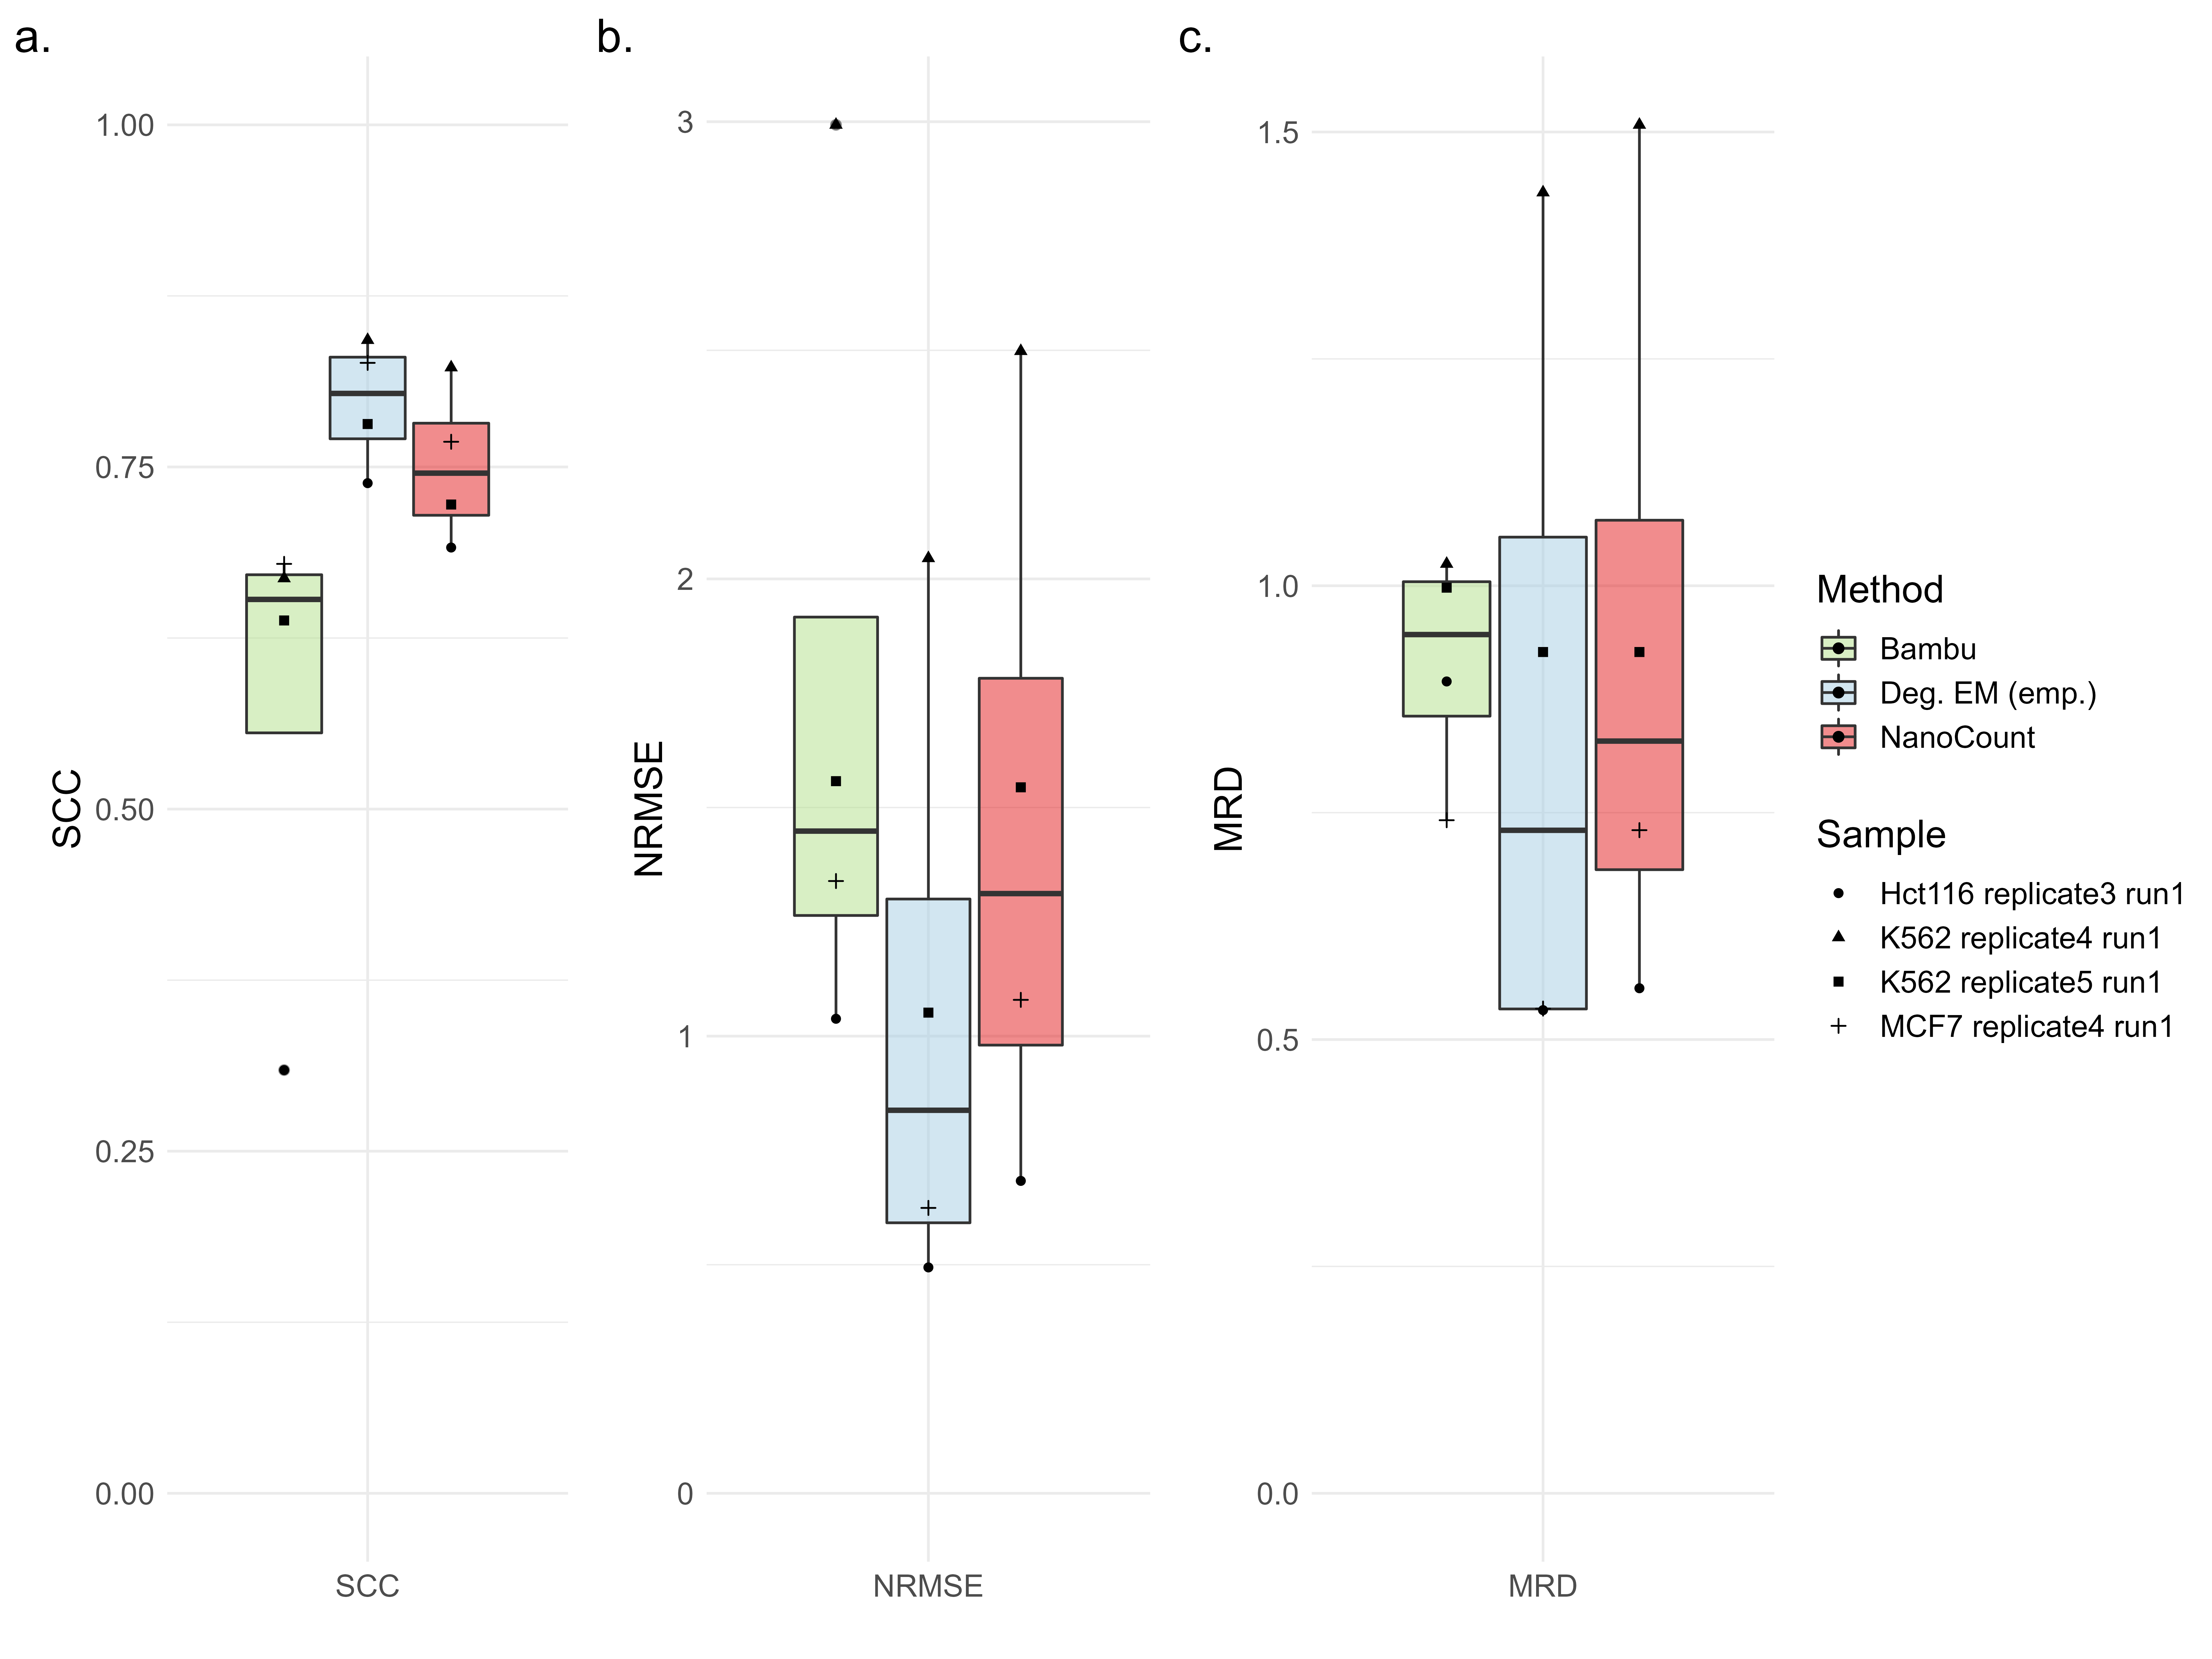
\includegraphics[width=\textwidth]{figures/sequin-metrics.png}
    \caption[SCC, NRMSE and MRD on RNA sequins in SG-NEx data]{SCC, NRMSE and MRD on RNA sequins in SG-NEx data. \textbf{a.} SCC, \textbf{b.} NRMSE and \textbf{c.} MRD for each of the three methods across four samples.}
    \label{fig:sequin-metrics}
\end{figure}

\begin{figure}[H]
    \centering
    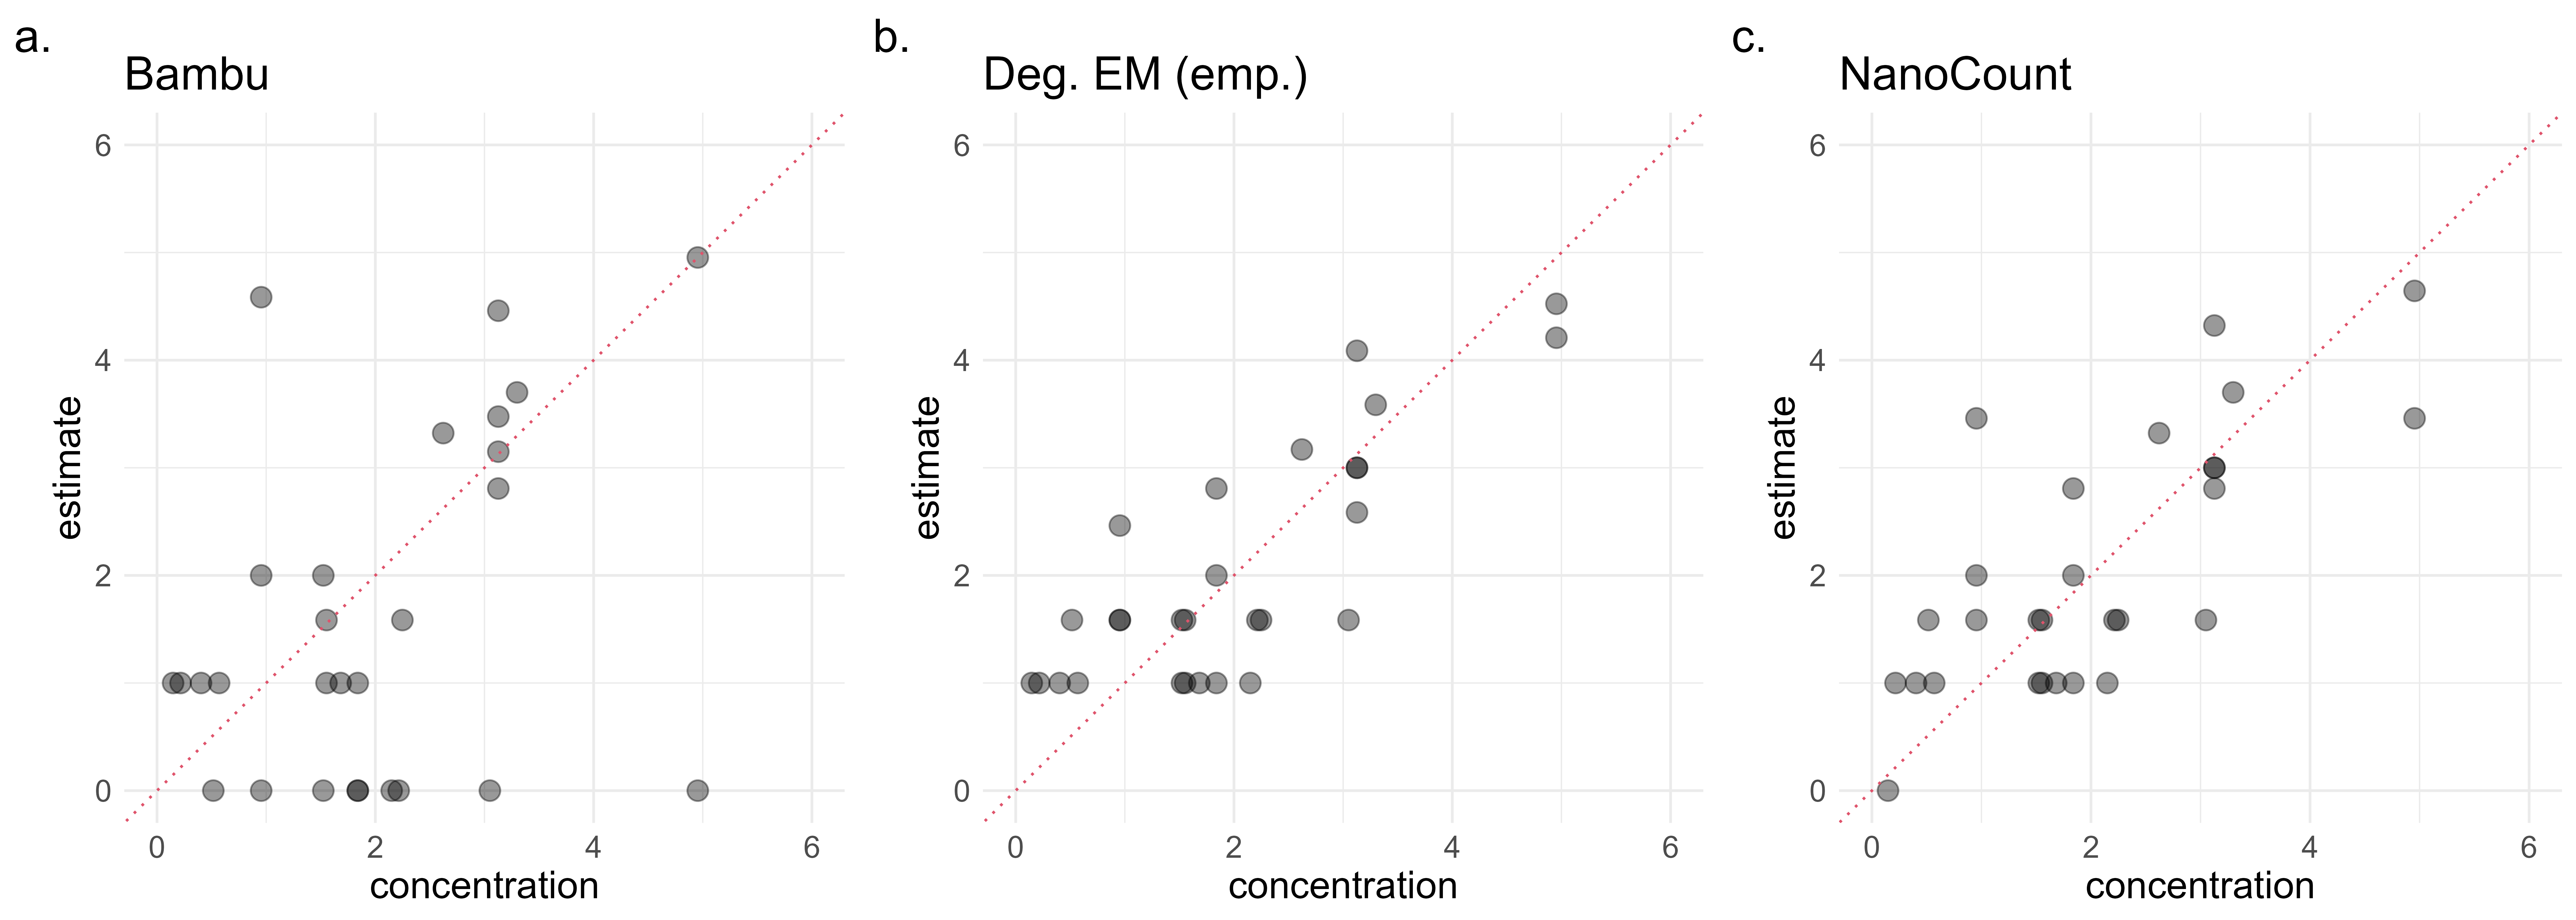
\includegraphics[width=\textwidth]{figures/sequin-scatter.png}
    \caption[Scatter plots on RNA sequins in SG-NEx data]{Scatter plots on RNA sequins in sample K562 replicate 5 run 1 for \textbf{a.} Bambu, \textbf{b.} Deg. EM (emp.) and \textbf{c.} NanoCount. Plots for rest of the samples are qualitatively similar.}
    \label{fig:sequin-scatter}
\end{figure}

\begin{figure}[H]
    \centering
    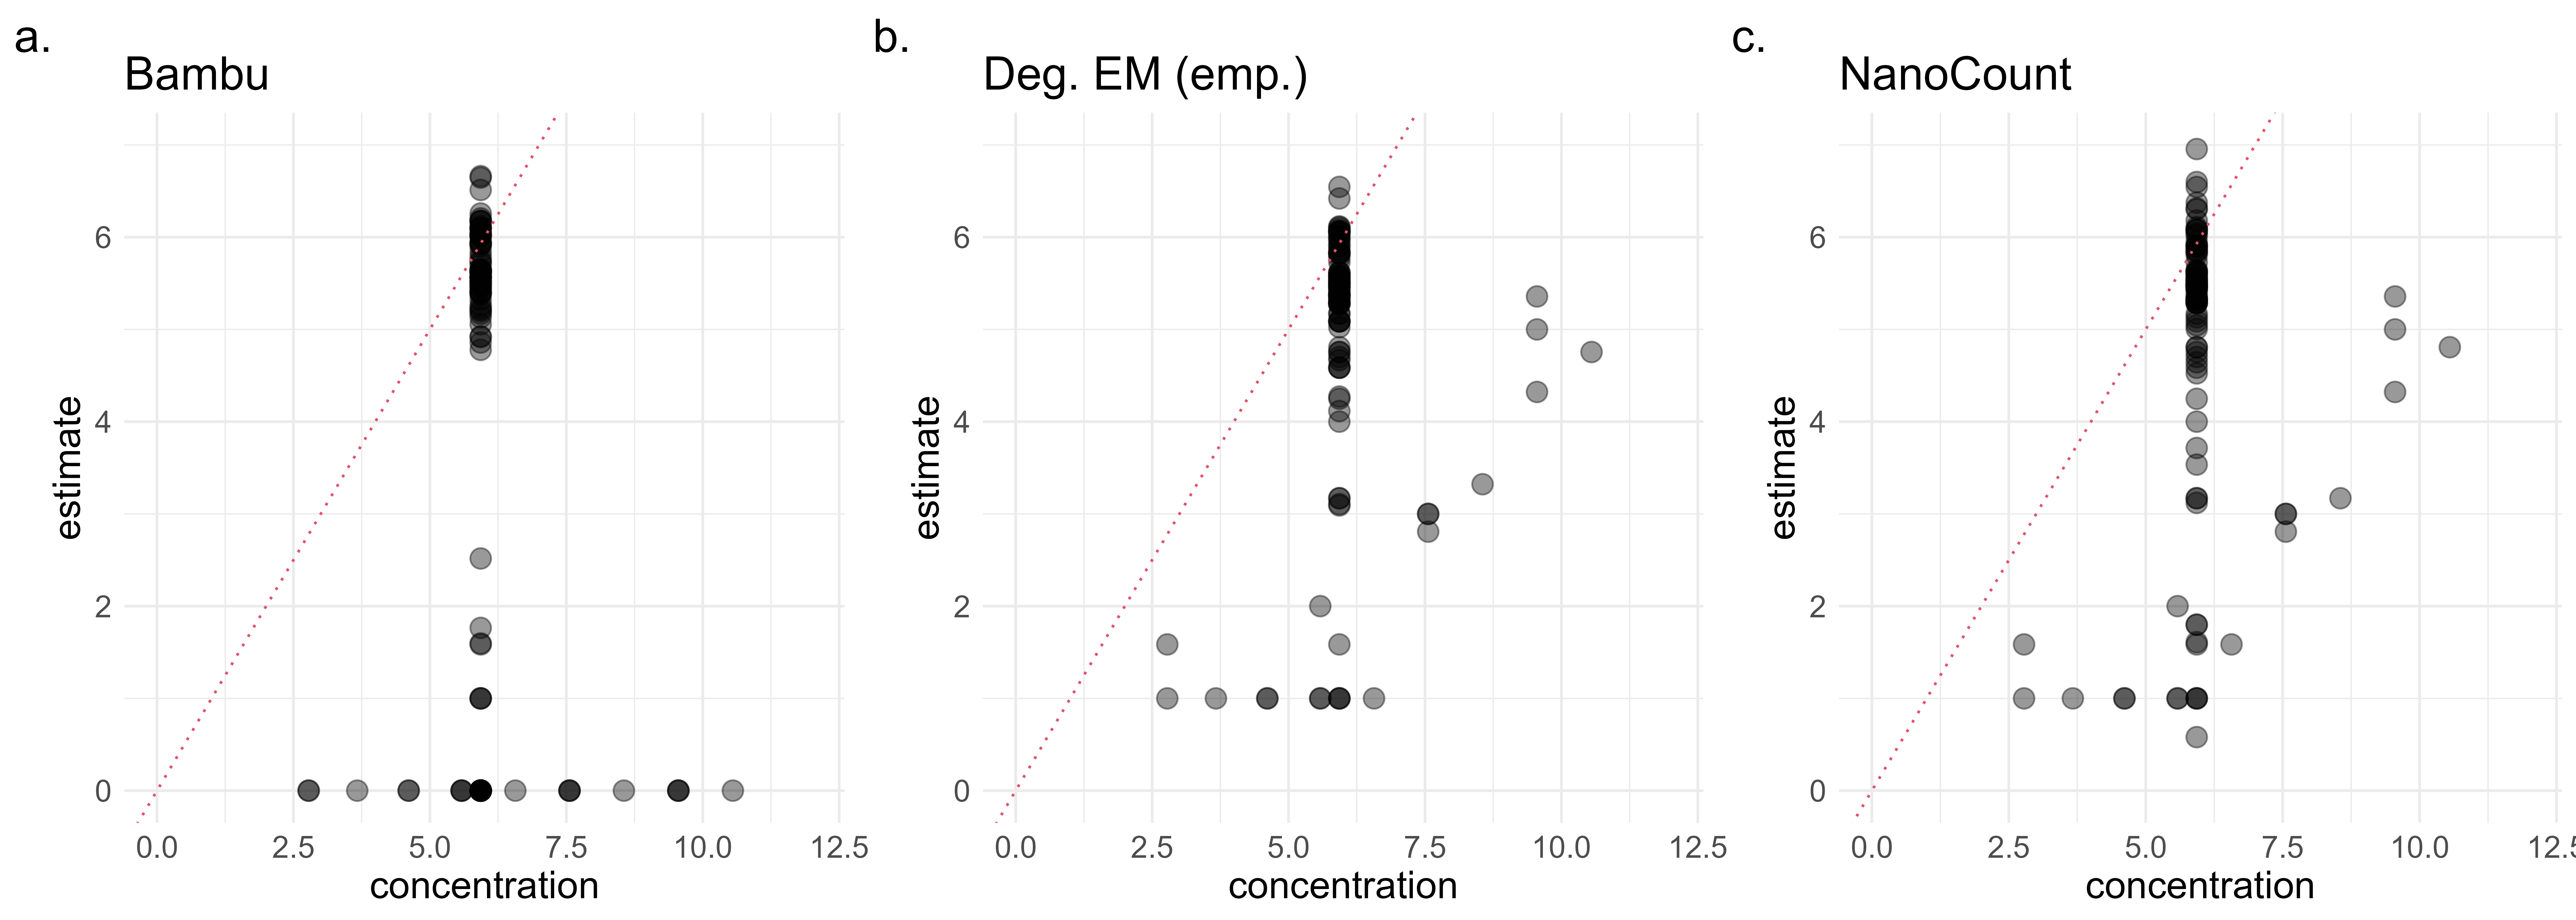
\includegraphics[width=\textwidth]{figures/lexogen-scatter.png}
    \caption[Scatter plots on SIRVs in SG-NEx data]{Scatter plots on SIRVs in SG-NEx data in H9 replicate 4 run 1 for \textbf{a.} Bambu, \textbf{b.} Deg. EM (emp.) and \textbf{c.} NanoCount. Plots for rest of the samples are qualitatively similar.}
    \label{fig:lexogen-scatter}
\end{figure}

\begin{figure}[H]
    \centering
    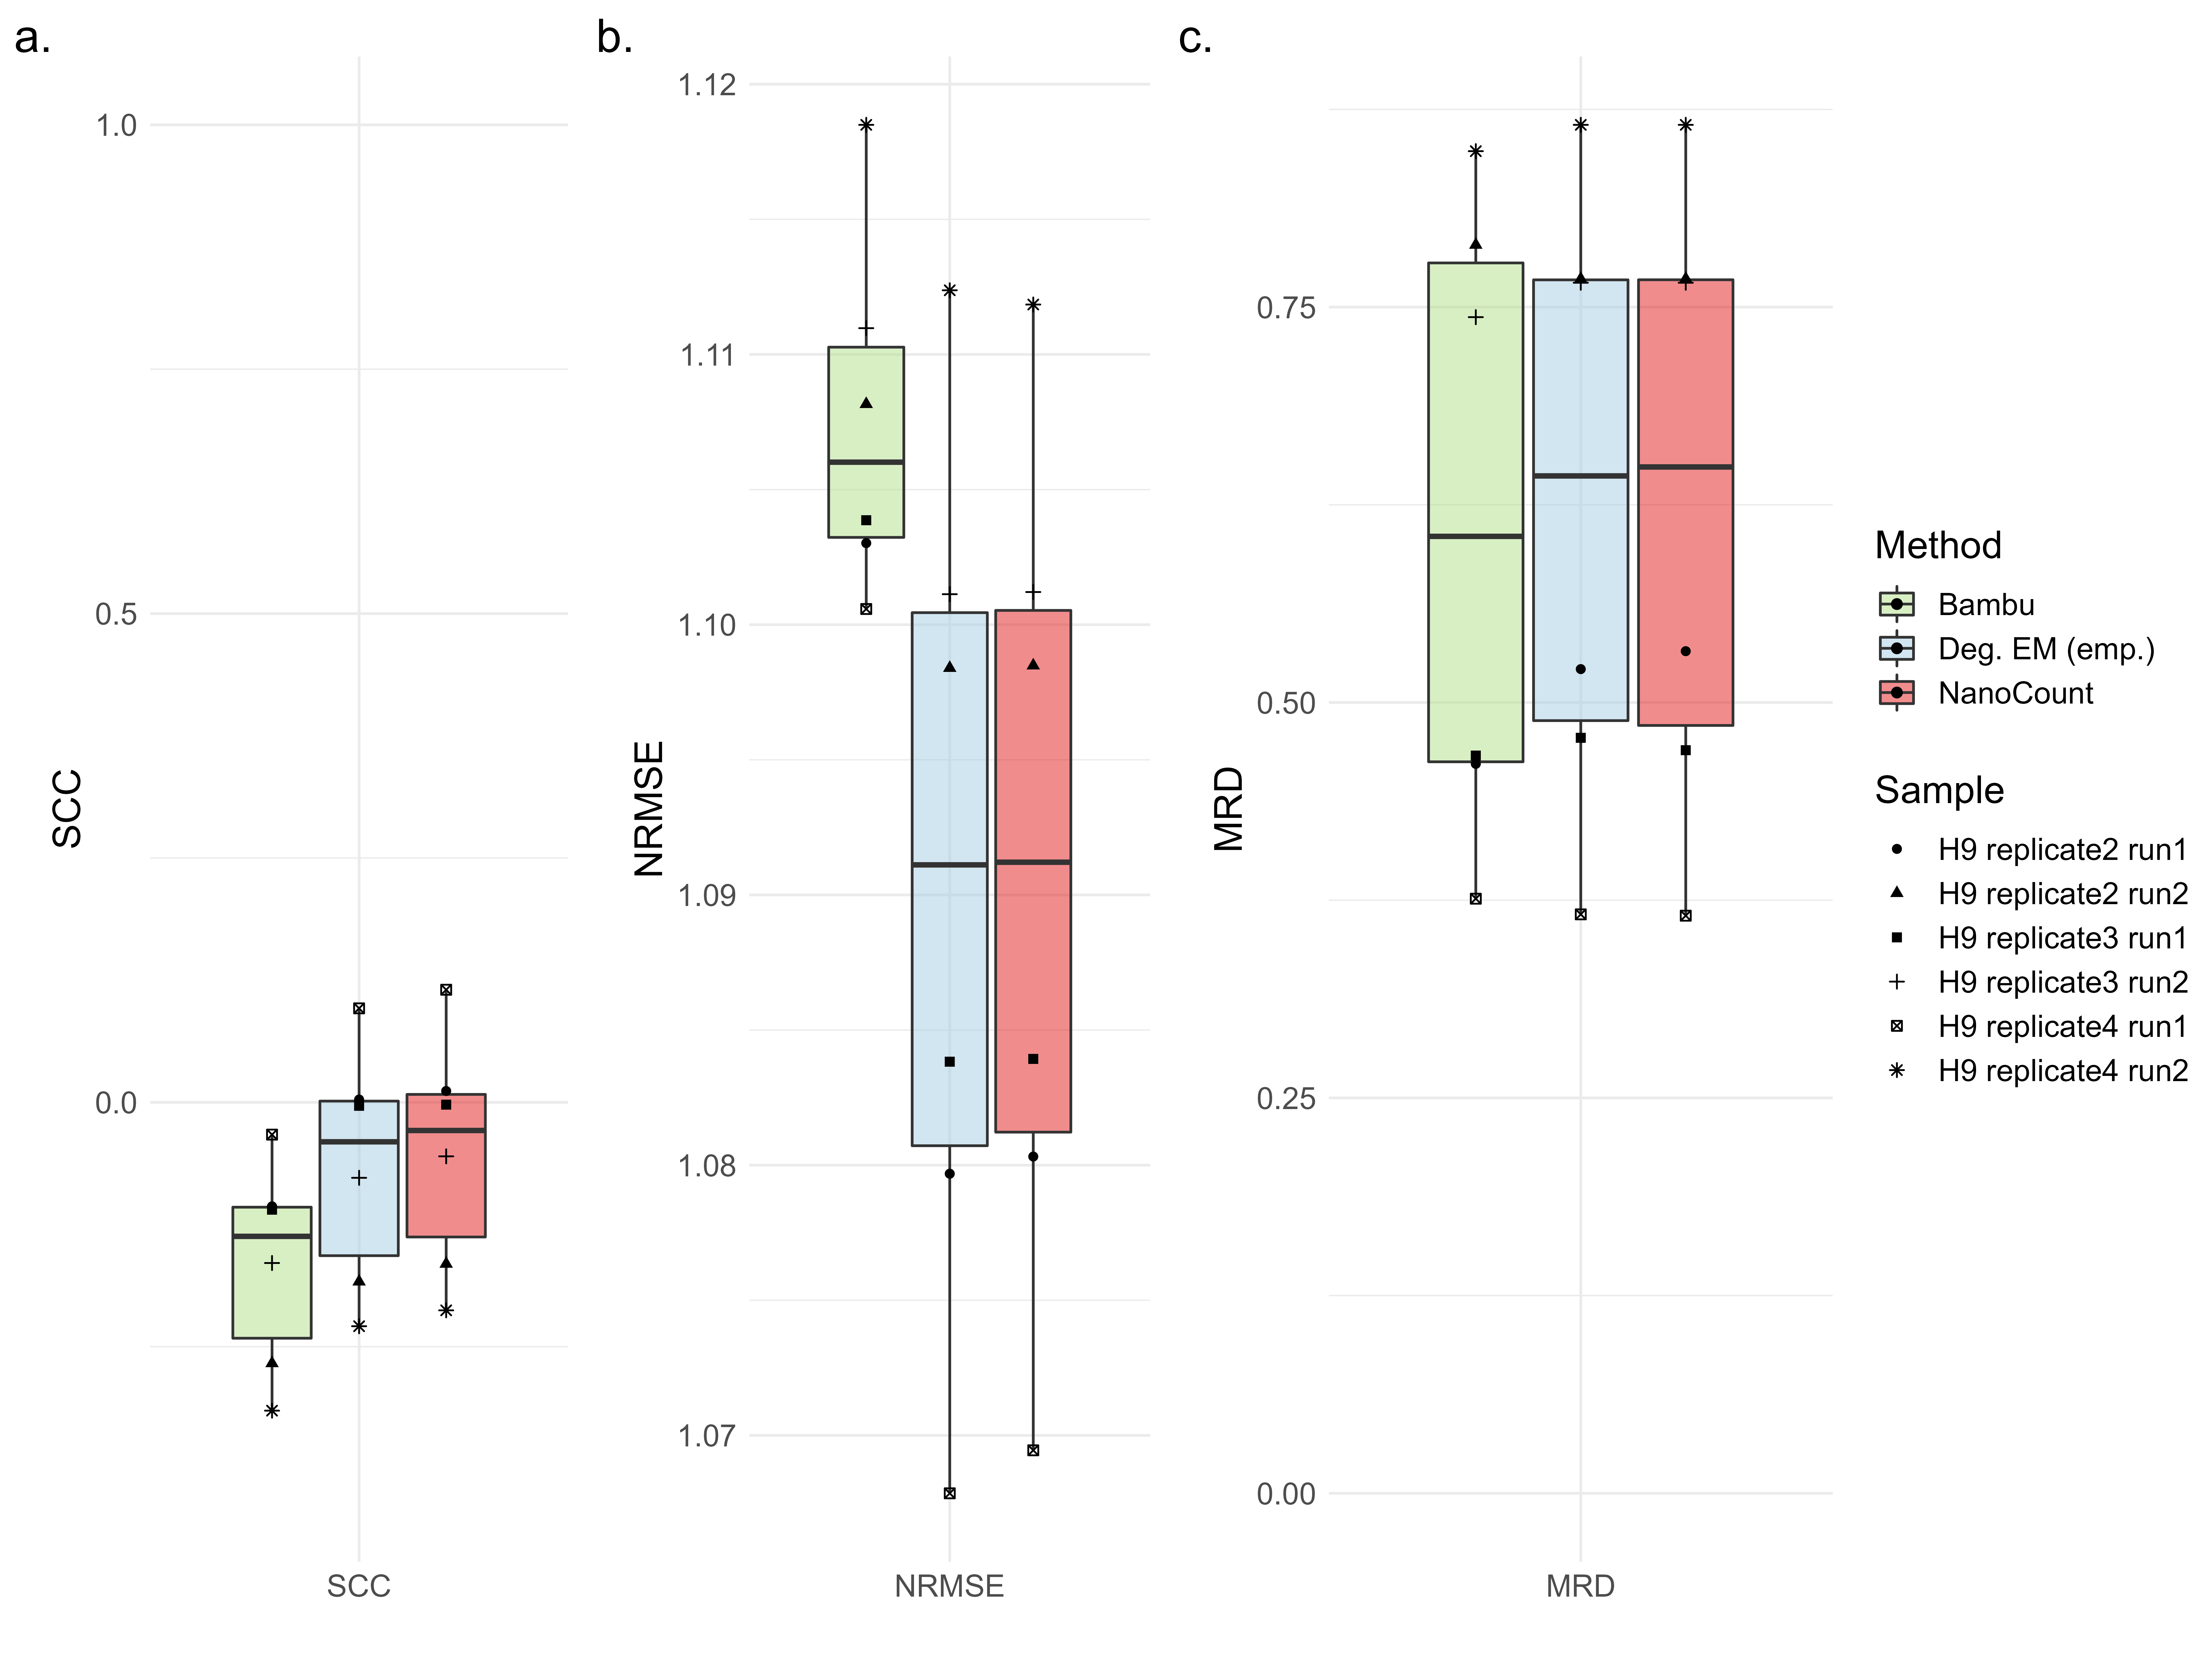
\includegraphics[width=\textwidth]{figures/lexogen.png}
    \caption[SCC, NRMSE and MRD on SIRVs in SG-NEx data]{SCC, NRMSE and MRD on SIRV-4 in SG-NEx data. \textbf{a.} SCC, \textbf{b.} NRMSE and \textbf{c.} MRD for each of the three methods across six H9 samples.}
    \label{fig:lexogen-metrics}
\end{figure}

In addition to the sequin spike-in samples, we examined the SIRV spike-ins in six H9 direct RNA-seq samples (Table \ref{tab-sgnex}). For all methods and across the samples, the abundance estimates for SIRVs did not reflect the supposed concentration (Fig. \ref{fig:lexogen-scatter}). However, the estimates obtained across the methods correlated well with each other (median of median pairwise SCC = 0.806, p-value $<$ 2.2e-16). This might suggest that the supposed SIRV concentrations do not accurately represent what is actually present in the samples, diminishing their utility as a control for RNA-seq in this context. Nevertheless, we computed the SCC, NRMSE and MRD across the six samples for each method (Fig. \ref{fig:lexogen-metrics}). The performance on all metrics is similar across the methods, but is unlikely to be informative due to reasons discussed above.   

\subsection{Reproducibilty measures}

Besides quantifying accuracy, we can also measure the reproducibility of abundance estimates for each method. We do so with the reproducibility metric (RM), which is a measure of the standard deviation of abundance estimates across replicates (Appendix \ref{ap:eval-metrics}). We use H9 samples in the SG-NEx data that were sequenced in two runs, with three replicates in each run (Table \ref{tab-sgnex}). Within each run, we calculated the RM across the replicates for each isoform called as expressed in at least one method and obtained the median reproducibiltiy metric (MRM) (Table \ref{tab-mrm}). For all methods, MRM in the first run was higher than that in the second by virtue of the number of isoforms the MRM was calculated over (Run 1 = 30,720, Run 2 = 21,536). In both runs, Deg. EM (emp.) achieved the lowest MRM suggesting higher reproducibility compared to NanoCount or Bambu. 

\begin{table}[htbp]
\centering
\begin{tabular}{|p{3cm}|p{2cm}|p{2cm}|}
\hline
Method & Run 1 & Run 2 \bigstrut\\
\hline
Deg. EM (emp.) & \textbf{0.904} & \textbf{0.812} \bigstrut\\
\hline
Bambu & 1.193 & 0.943 \bigstrut\\
\hline
NanoCount & 0.943 & 0.816 \bigstrut\\
\hline
\end{tabular}%
\caption[MRM across different runs for SG-NEx data]{MRM across different runs for SG-NEx H9 samples.}
\label{tab-mrm}%
\end{table}%

The incorporation of bias modeling in Deg. EM improves reproducibility. We can infer this by comparing the MRMs obtained by Deg. EM and NanoCount since the latter is most comparable to our Deg. EM. By modeling the bias, read-to-isoform assignment is improved across replicates with potentially different degradation rates, thus stabilising variance in abundance estimates across the replicates.       

\subsection{Comparisons of estimated degradation}

Lastly, we compare the estimated average degradation rates obtained by Bambu and Deg. EM (emp.) across samples from four cell lines. We note that we do not expect the absolute values of the degradation rates to be similar; rather, we expect the estimates to be linearly related. Indeed, by regressing the degradation rate estimates from Bambu against Deg. EM (Fig. \ref{fig:real-deg-rate}) in a linear model, we find that the linear relationship is significant (p-value = 2.63e-05, adjusted $R^2$ = 0.890). Even though the sample size here is small, the concordance between the degradation rates estimated by Bambu and Deg. EM (emp.) on real data provides a useful sanity check for our model.

\begin{figure}
    \centering
    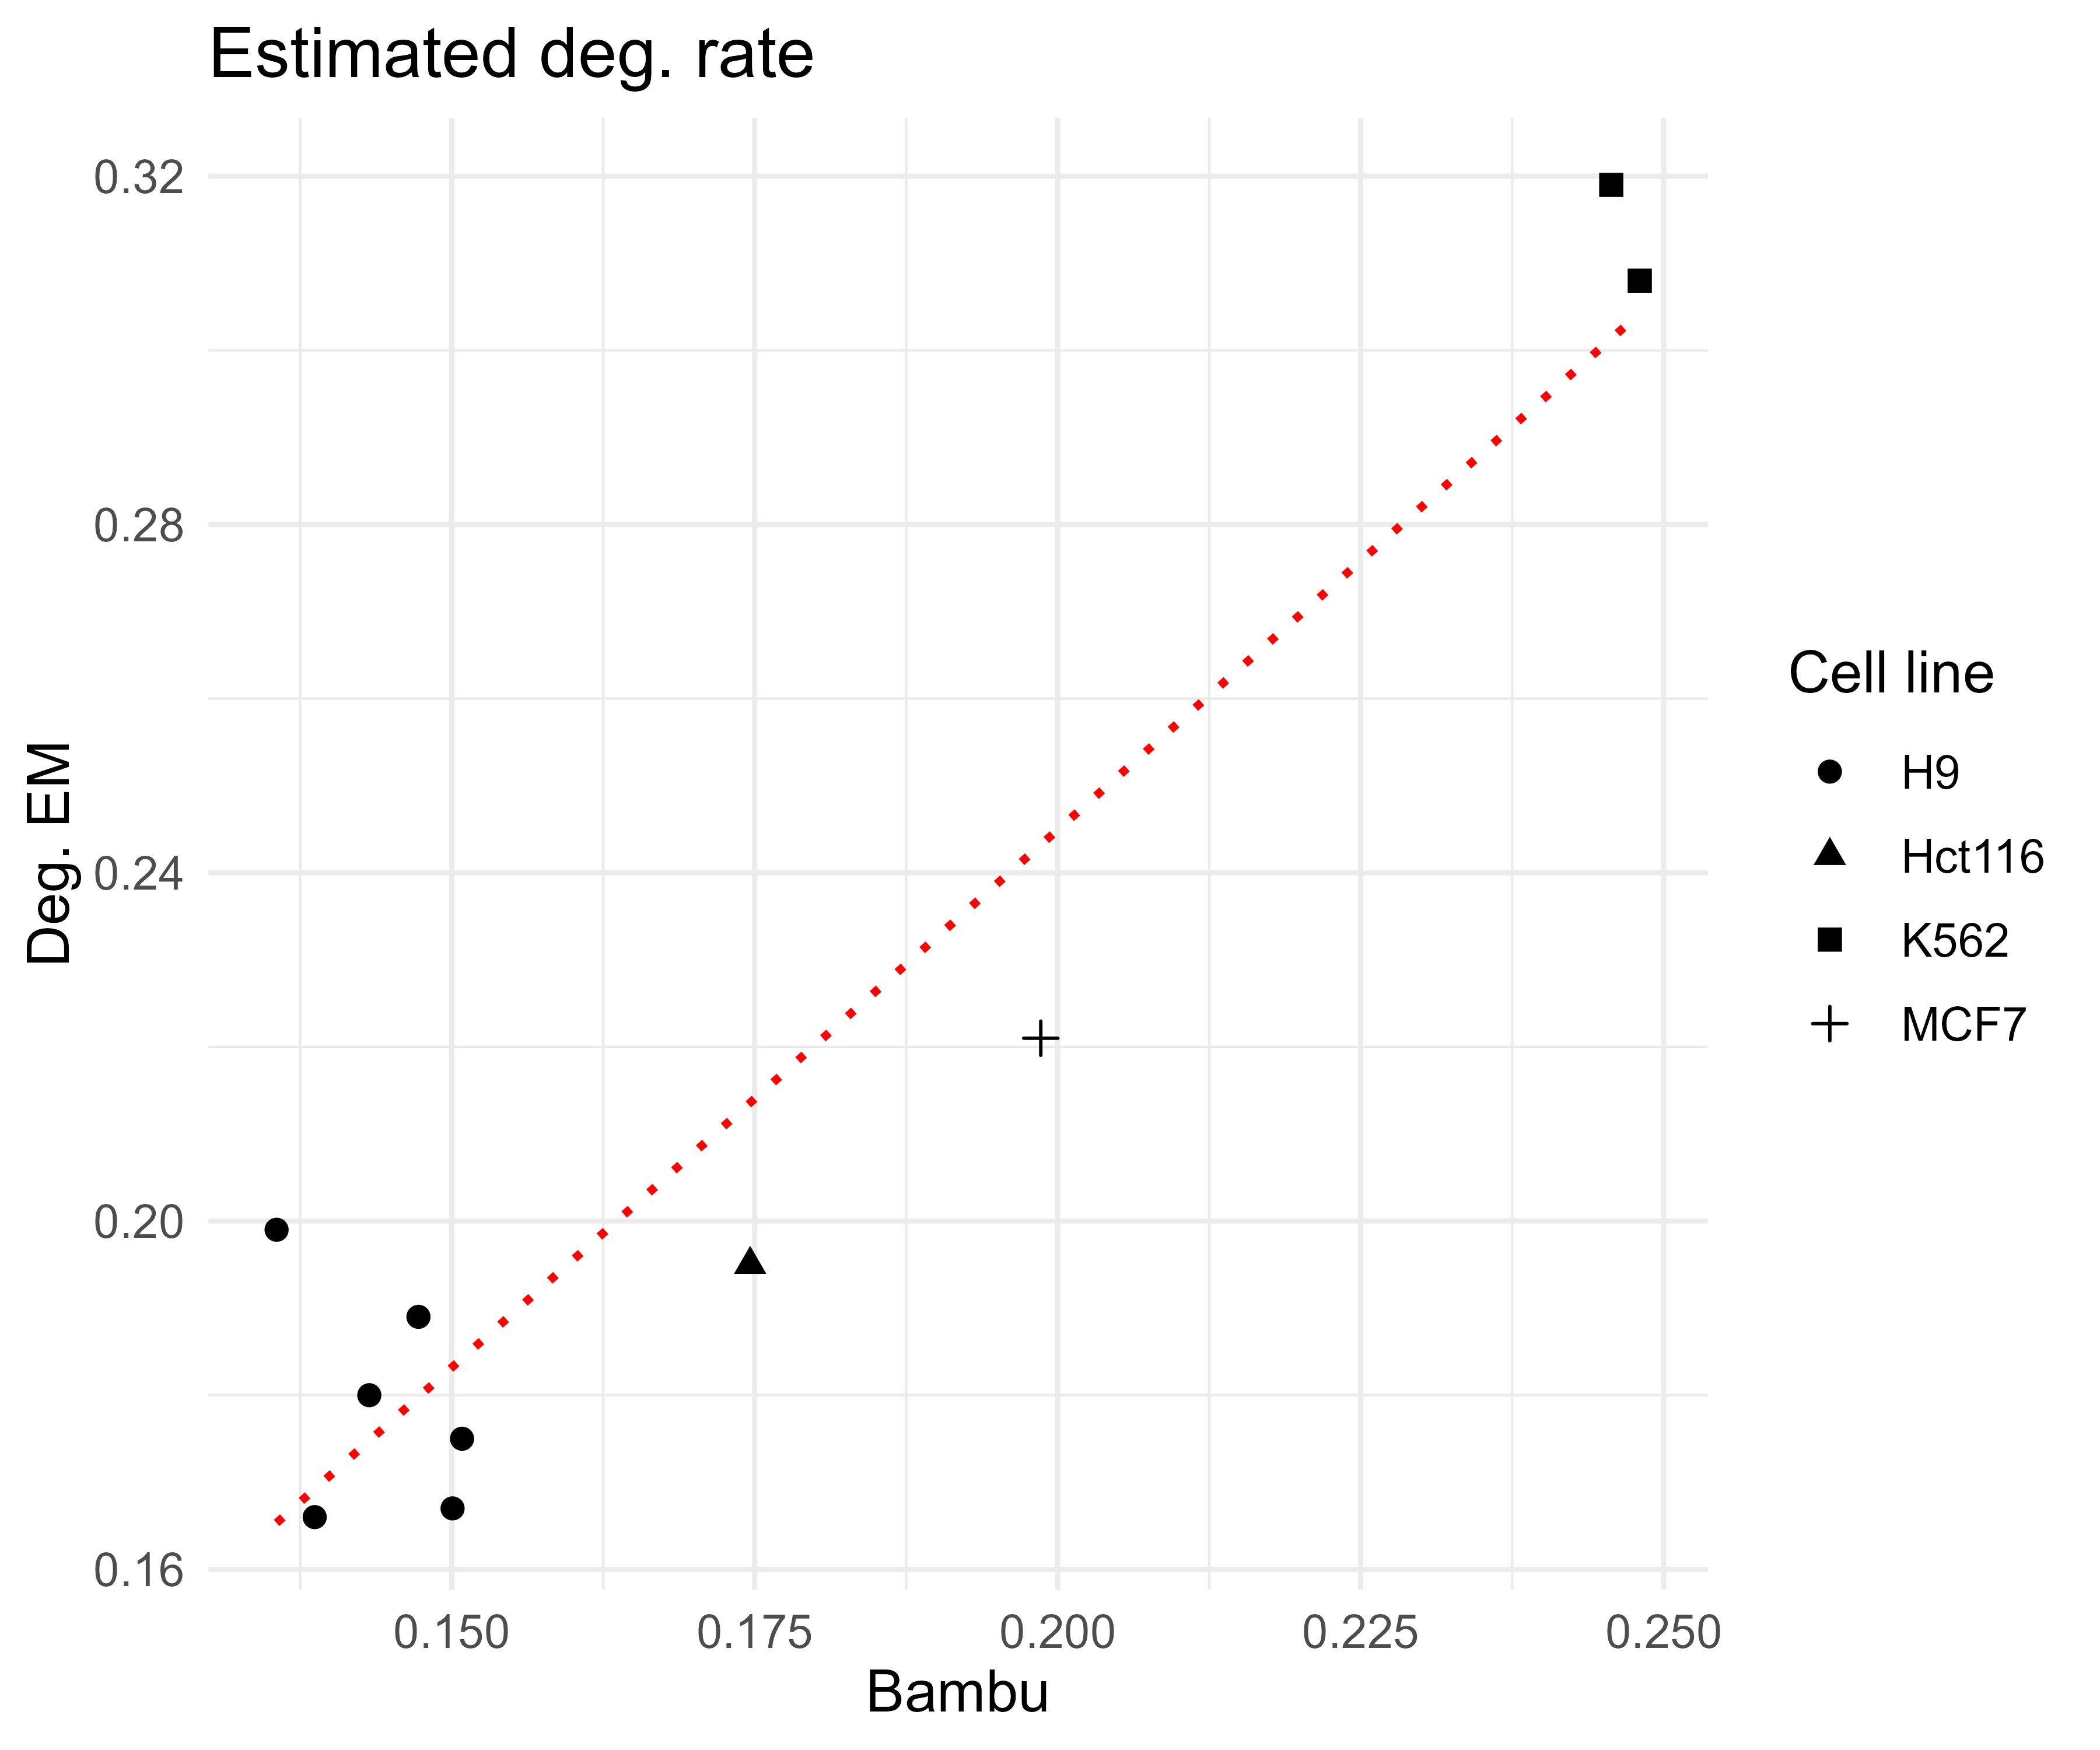
\includegraphics[width=0.65\textwidth]{figures/real-deg-rate.png}
    \caption[Comparison of estimated degradation rates on SG-NEx data]{Comparison of estimated degradation rates on SG-NEx data across four cell lines.}
    \label{fig:real-deg-rate}
\end{figure}

\section{Discussion}

In this chapter, we evaluated our model and inference algorithm (Deg. EM) on simulated datasets with known constant degradation rates and real datasets with sequencing spike-ins from the SG-NEx project. First, we compared the exact and empirical variations of our model, finding that they perform comparably in the range of realistic degradation rates. 

Next, we benchmarked Deg. EM against Bambu, Bambu without bias, FLAIR and NanoCount. We showed on simulated datasets that Deg. EM achieves the best performance on SCC, NRMSE and MRD compared to existing methods. In particular, methods that do not model for bias perform poorly on subset isoforms. The results obtained on real datasets with spike-ins were similar, with Deg. EM showing comparable, if not slightly better performance compared to NanoCout and Bambu. We also found that the variance in estimates obtained by Deg. EM was lower compared to those of other methods across replicates, showing that modeling degradation can help increase reproducibility \textit{in silico}.   